\documentclass[twocolumn]{article}
\usepackage[utf8]{inputenc}
\usepackage{graphicx}
\usepackage{textcomp}
\usepackage{fullpage}
\usepackage{float}
\usepackage{listings}
\usepackage{verbatim}

\title{Deep Learning Assignment 2}
\author{Nikita Teplitskiy}

\begin{document}
\maketitle
\section{Introduction}
This assignment was completed using the Keras library by constructing a perceptron with two hidden layers, each containing 16 neurons. The model is able to reliably classify its training data set with perfect accuracy and performs well on unfamiliar data. The form of the perceptron function can be seen in Figure 1; its outline was generated by plotting a selection of points from the X/Y plane on a contour plot.

\begin{figure}[H]
    \centering
    \hspace*{-1cm}    
    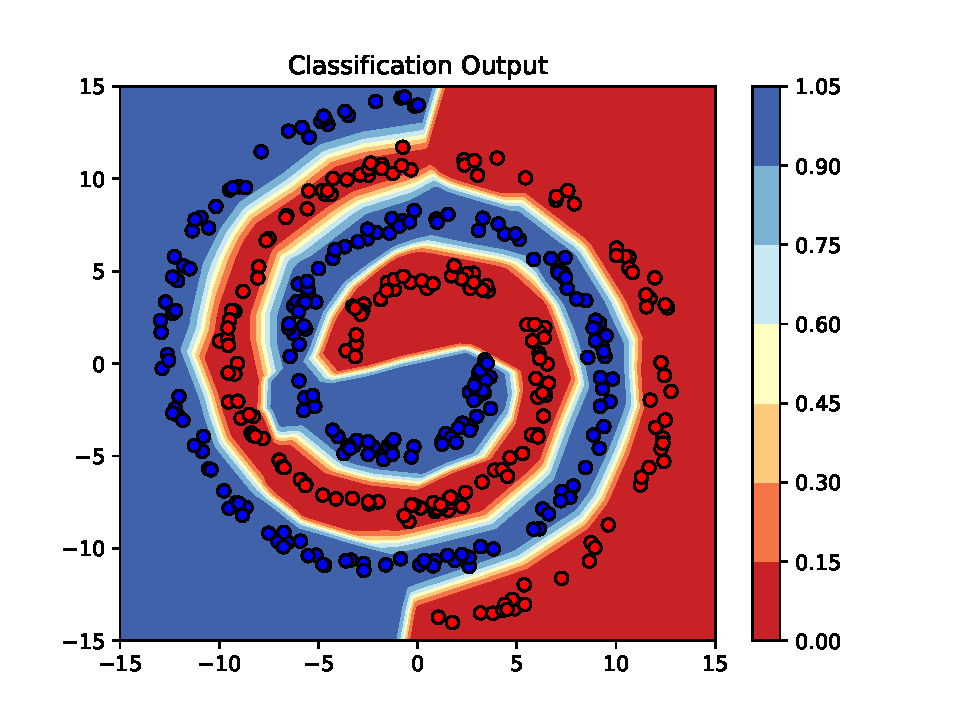
\includegraphics[width=0.6\textwidth]{result.pdf}
    \caption{Output of multilayer perceptron classifier}
\end{figure}

\begin{figure}[H]
    \centering
    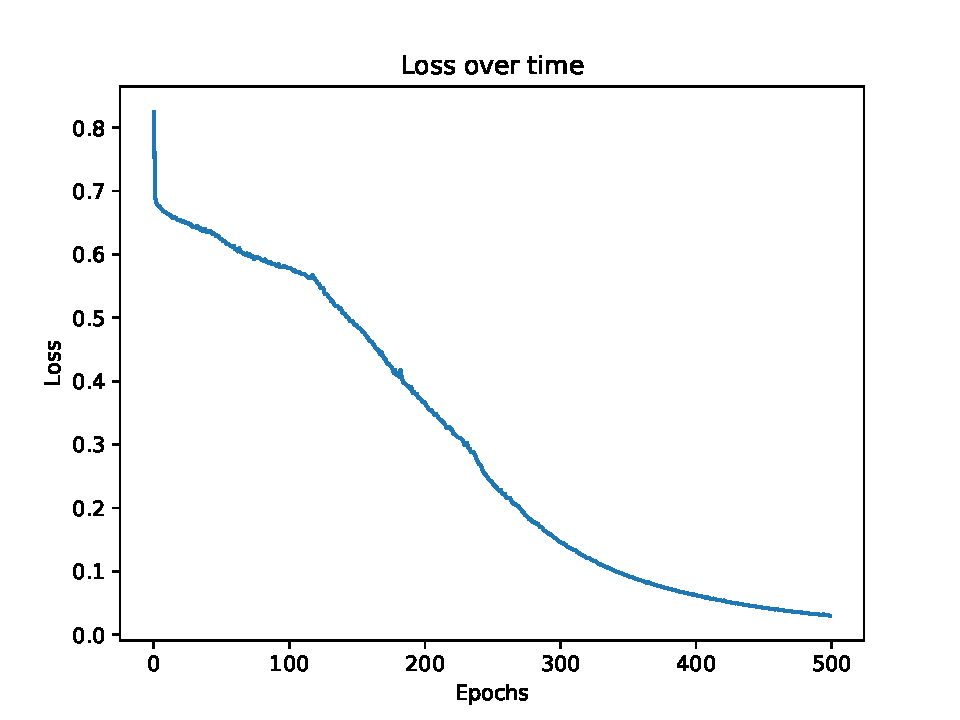
\includegraphics[width=0.6\textwidth]{loss.pdf}
    \caption{Loss over training iterations}
\end{figure}

\begin{figure}[H]
    \centering
    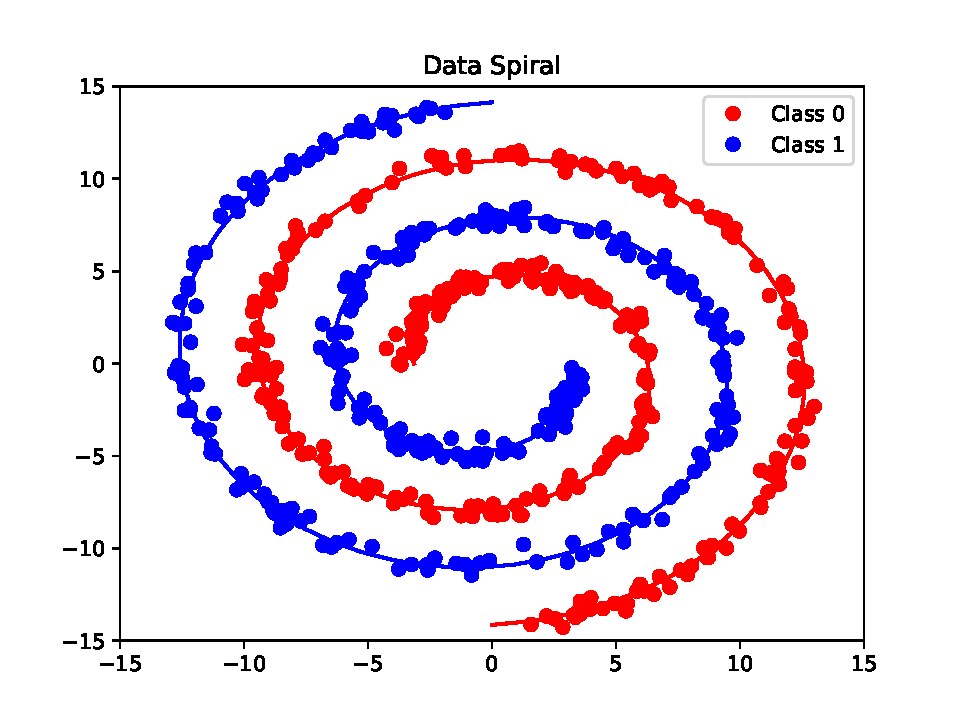
\includegraphics[width=0.6\textwidth]{data.pdf}
    \caption{Starting Data}
\end{figure}

\newpage
\onecolumn
%\verbatiminput{a2.py}

\newpage
\section{Code}
\lstinputlisting[language=Python]{a2.py}


\end{document}
